\section{Blocking Design}
\begin{frame}
  \begin{center}
    {\bf Part II - Blocking Design}
  \end{center}
\end{frame}

\begin{frame}{Completely Randomized Design (CRD)}
  Until now, we studied the following situation:
  \begin{itemize}
    \item One input factor (for example, algorithm type)
    \item One response variable (for example, solution speed)
    \item An {\bf homogeneous experimental condition}.
  \end{itemize}\bigskip

  \begin{block}{Homogeneous experimental condition}
    This means that the experiment environment is guaranteed to be the same
    for all observations, and there are no significant error sources.
  \end{block}\bigskip

  In this situation, we execute the experiment in {\bf random order} to
  guarantee that any error sources are equally distributed.
  We call this a {\bf Completely Randomized Design (CRD)}
\end{frame}

\begin{frame}{Block Design}

  {\bf Noise / Nuisance Factors} are input variables that can have a significant impact in
  the experiment output, but they are not relevant to the scientific question.\bigskip

  In a previous lecture, we discussed the use of {\bf Pairing} to remove the
  effect of \emph{one} noise factor. {\bf Blocking} is the generalization of the
  Paired Design approach for multiple noise factors.\bigskip

  \begin{block}{Block Design vs Completely Randomized Design}
    We use Randomization (CRD) to prevent the effect of \emph{unknown} noise factors in our experiment.
    \bigskip

    We use Blocking or Pairing when we know from the beginning that certain factors affect the output
    variable, but for some reason we are not interested in their effects.
  \end{block}
\end{frame}

\subsection{Example Problem}
\begin{frame}{Example of Block Design}{Algorithm Comparison}

  A student decides to compare a standard optimization algorithm against
  size variants to solve a certain family of Vehicle Routing Problems (VRPs).
  \bigskip

  He wants to know if any variant returns a systematically lower cost value,
  when applied to 180 problem instances. These instances can be divided in
  {\bf 36 groups}, with 5 similar instance in each group.


  \begin{columns}
    \column{.8\textwidth}
    \begin{block}{Experiment Design Variables}
      \begin{itemize}
        \item confidence: $\alpha = 0.05$
        \item power: $\pi = 1 - \beta = 0.8$
        \item minimally interesting effect: $\delta^* = 50$
      \end{itemize}
    \end{block}
    \column{.2\textwidth}
    
\includegraphics[width=1\textwidth]{../img/phdStudent.png}
    \ppagenote{PhD Student Image: PhD Comics by Jorge Cham, http://www.phdcomics.com/comics/archive.php?comicid=1139}
  \end{columns}
\end{frame}

\begin{frame}{Example of Block Design: Factors and levels}
  For this problem, we can identify the following variables:
  \begin{itemize}
    \item {\bf Input Factor}: Algorithm; {\bf Levels:} Original and 6 variants;
    \item {\bf Return Variable}: Cost; {\bf Levels:} Integer value;
    \item {\bf Noise Factor}: Instance type; {\bf Levels:} 36 groups;
  \end{itemize}\bigskip

  If we employ a CRD (ignoring or randomizing the Noise Factor), the difference
  in result among Instance types would have an effect in the residual, and possibly mask
  the difference between algorithms.\bigskip

  To avoid this, we organize the experiment in 36 blocks (one block per level of
  the Noise Factor), and randomize the execution of all 7 algorithms inside each block.
  This is the {\bf Randomized Complete Block Design (RCBD)}
\end{frame}

\begin{frame}{Assumptions of the RCBD}
  The RCBD assumes the following characteristics for the experiment:
  \begin{enumerate}
    \item one replicate per block;
    \item the blocks are independent;
    \item randomization inside the block is independent;
  \end{enumerate}\bigskip

  These assumptions are important. If we fail to guarantee the
  independence between the blocks (for example, some of the blocks are dependent),
  we introduce something called {\bf pseudoreplication}, which may result in
  an inflation of type-I error.
\end{frame}

\begin{frame}{Example: Pre-processing the data}
  In the algorithm example, we obtain the following experimental data:
  \begin{itemize}
    \item 7 algorithm variants,
    \item 180 total problem instances, 36 instance group (5 instances per group)
    \item 30 repetitions, per algorithm, per instance (7x30x180 = 37800 observations)
  \end{itemize}\bigskip

  However, as explained in the last slide, the RCBD requires {\bf 1 replicate per block}.
  To satisfy this requirement, we pre-process the data as follows:
  \begin{itemize}
    \item The performance of each algorithm, per instance, is averaged (average of 30 repetitions)
    \item The performance of each algorithm, per group, is averaged (average of 5 instances)
  \end{itemize}
  This gives us 36 observations per algorithm (1 observation per block)
\end{frame}

\begin{frame}[fragile]{Example: Pre-processing the data (R code)}

{\smaller
\begin{verbatim}
> data <- read.table("../data files/algo.csv", header = TRUE)
# Aggregate data (algorithm means by instance group)
> aggdata <- with(data, aggregate(x   = Result, by  = list(Algorithm, Group),
                                  FUN = mean))
# Rename columns and coerce factor variables
> names(aggdata) <- c("Algorithm", "Instance_Group", "Y")
> for (i in 1:2) aggdata[, i] <- as.factor(aggdata[, i])
> levels(aggdata$Algorithm) <- c("Original", unlist(lapply(X   = "Mod",
                                               FUN = paste0, 1:6)))
> summary(aggdata)
    Algorithm  Instance_Group       Y
 Original:36   1      :  7    Min.   : 227.3
 Mod1    :36   2      :  7    1st Qu.: 440.0
 Mod2    :36   3      :  7    Median : 756.8
 Mod3    :36   4      :  7    Mean   : 821.0
 Mod4    :36   5      :  7    3rd Qu.:1020.5
 Mod5    :36   6      :  7    Max.   :2743.6
 Mod6    :36   (Other):210$
\end{verbatim}}
\end{frame}

\begin{frame}[fragile]{Example: Pre-visualization of the Data (R code)}

{\smaller
\begin{verbatim}
> p <- ggplot(aggdata, aes(x = Instance_Group, y = Y,
                           group = Algorithm, colour = Algorithm))
> p + geom_line(linetype=2) + geom_point(size=5)
\end{verbatim}
}

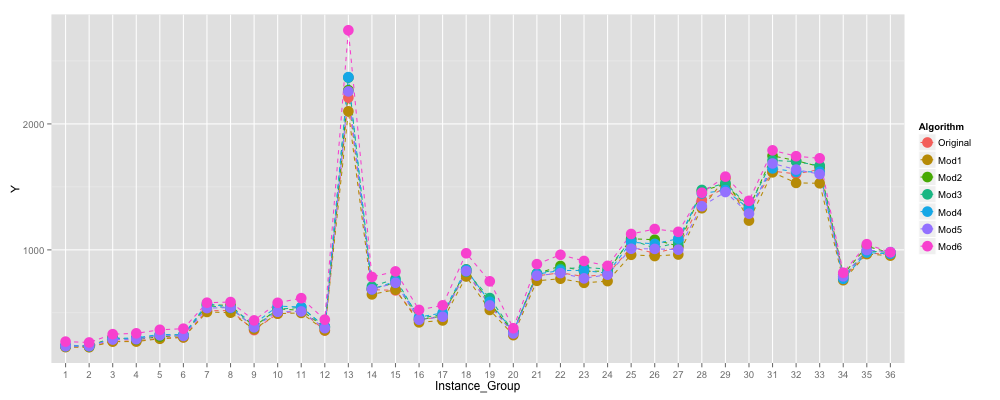
\includegraphics[width=.9\textwidth]{../img/algo_lineplot.png}
\end{frame}

\begin{frame}[fragile]{Statistical Analysis of the CRBD}

The Statistical analysis of the CRBD is similar to the ANOVA analysis we
studied in a previous class. For a derivation of the model, see Campelo in the
recommended readings. \bigskip

However, note that the number of observations is based on the number of blocks
and treatment levels.

{\smaller
\begin{verbatim}
# Anova Model: Treatments+Blocks
> model <- aov(Y~Algorithm+Instance_Group, data=aggdata)

> summary(model)
                Df   Sum Sq Mean Sq F value Pr(>F)
Algorithm        6   359949   59991   41.75 <2e-16 ***
Instance_Group  35 60438639 1726818 1201.86 <2e-16 ***
Residuals      210   301725    1437
---
Signif. codes:  0 '***' 0.001 '**' 0.01 '*' 0.05 '.' 0.1 ' ' 1
\end{verbatim}
}
\end{frame}


\begin{frame}[fragile]{Statistical Analysis of the CRBD -- Residuals}

{\smaller
\begin{verbatim}
> summary.lm(model)$r.squared          # It's important to check the residuals
[1] 0.9950618                          # for anomalies. For example, here
> par(mfrow = c(2, 2))                 # The residual plot shows several outliers
> plot(model, pch = 20, las = 1)       # that could affect the result.
\end{verbatim}}
\centering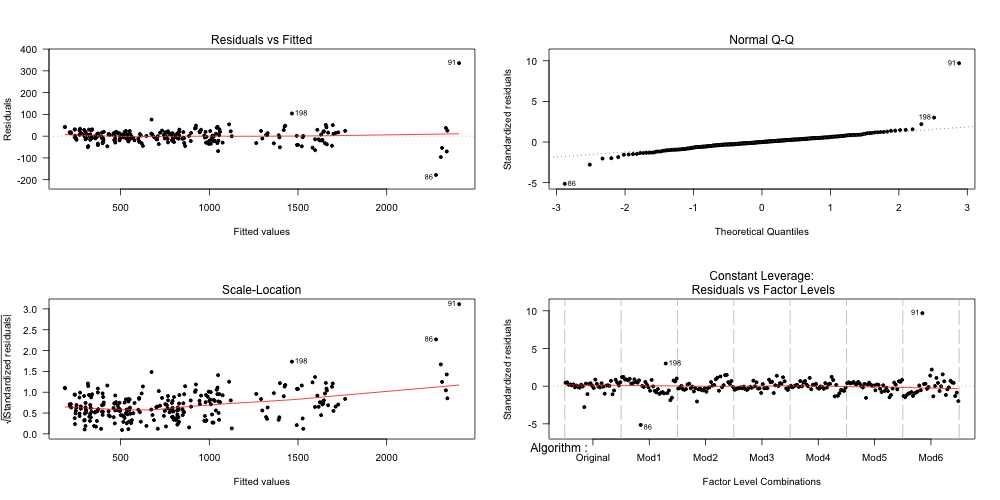
\includegraphics[width=.7\textwidth]{../img/algo_res1.png}
\end{frame}

\begin{frame}[fragile]{Statistical Analysis of the CRBD -- Log Transformation}

An analysis of the residual model showed some irregularities in the
residual plot, so we try a log transformation on the response variable
to see if we can smooth it out.

{\smaller
\begin{verbatim}
# Trying with log-transformed response variable
> model2 <- aov(log(Y)~Algorithm+Instance_Group, data=aggdata)

> summary(model2)
                Df Sum Sq Mean Sq F value Pr(>F)
Algorithm        6   0.60  0.1002   120.4 <2e-16 ***
Instance_Group  35  89.92  2.5690  3089.0 <2e-16 ***
Residuals      210   0.17  0.0008
\end{verbatim}
}
\end{frame}

\begin{frame}[fragile]{Statistical Analysis of the CRBD -- Log Transformation}

{\smaller
\begin{verbatim}
> summary.lm(model2)$r.squared         # The log transformation smoothed out
[1] 0.9980742                          # the outliers from our CRBD model.
> par(mfrow = c(2, 2))                 #
> plot(model2, pch = 20, las = 1)      #
\end{verbatim}}
\centering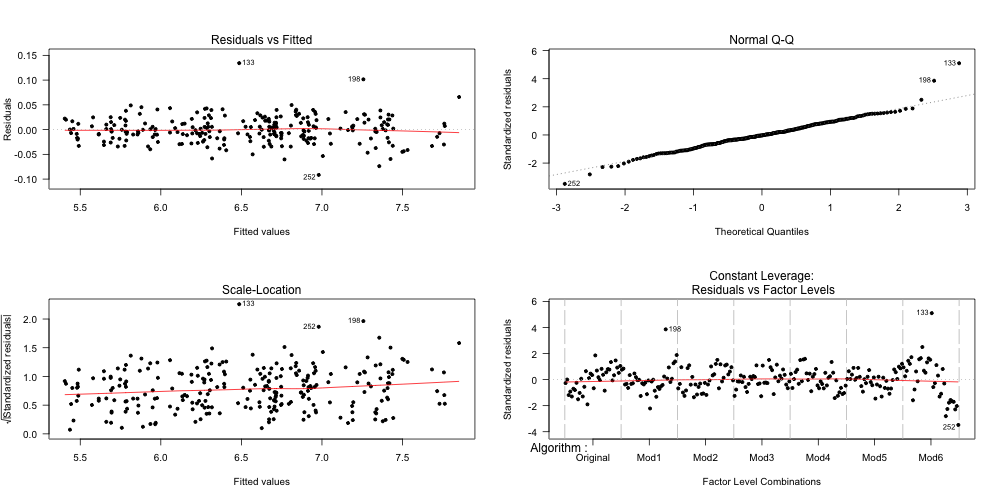
\includegraphics[width=.7\textwidth]{../img/algo_res2.png}
\end{frame}

\begin{frame}{Statistical Analysis of the CRBD -- final comments}
  The post-hoc analysis of the CRBD follows the same principles of the
  post-hoc analysis of the ANOVA.\bigskip

  \begin{itemize}
    \item The type and number of comparisons should be defined a priori.
    \begin{itemize}
      \item In this example, two-sample comparisons between the original algorithm and each variant would be appropriate.
    \end{itemize}
    \item The number of observations should be based on the number of blocks.
    \item Alpha-correction for the paired observations should be applied as necessary.
  \end{itemize}
\end{frame}

\subsection{}
\begin{frame}{Further Reading}
  You should do further reading for these two models that are closely related to the CRBD:
  \begin{itemize}
    \item "Incomplete Block Design" -- When some of the observations (blocks) are missing;
    \item "Generalized Block Design" -- When each block has multiple replicates;
  \end{itemize}
\end{frame}
